\begin{statementbox}
\textbf{C094\quad 共焦椭圆与双曲线的四个公共点及坐标}

设椭圆 $E$ 与双曲线 $H$ 为\textbf{非退化、实、具有同一对焦点}的曲线，
取公共焦点 $F_1=(-c,0),F_2=(c,0)$，$c>0$。分别记
椭圆半长轴 $a_E$、半短轴 $b_E$，双曲线实半轴 $a_H$、虚半轴 $b_H$。
\[
\begin{gathered}
 a_E>c>a_H>0,\qquad
 b_E^2=a_E^2-c^2>0,\quad b_H^2=c^2-a_H^2>0,\\
 E:\ \frac{x^2}{a_E^2}+\frac{y^2}{b_E^2}=1,\qquad
 H:\ \frac{x^2}{a_H^2}-\frac{y^2}{b_H^2}=1.
\end{gathered}
\]
\begin{center}
% C094 precise confocal ellipse/hyperbola diagram
% E: x^2/16+y^2/12=1 ; H: x^2-y^2/3=1 ; F1=(-2,0),F2=(2,0)
% Intersections: (+/-2, +/-3). Geometry controlled by exact equations.
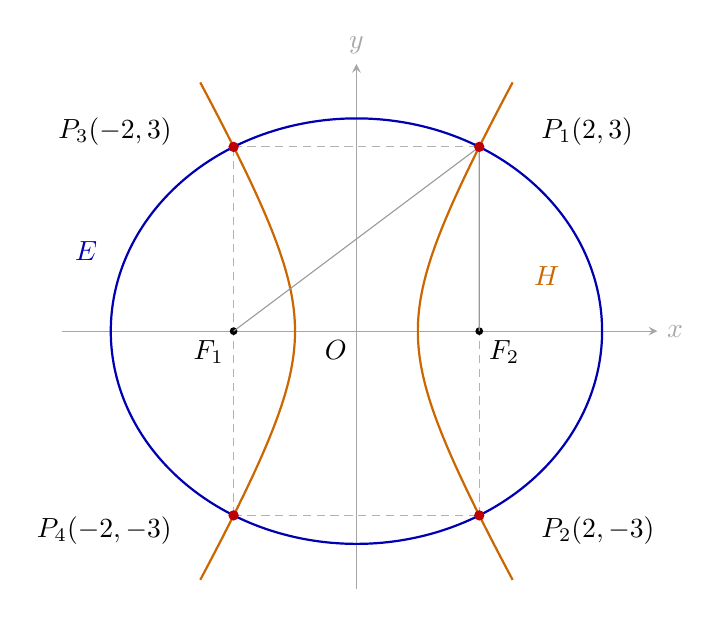
\begin{tikzpicture}[scale=0.78,>=stealth]
  \draw[->,gray!70] (-4.8,0)--(4.9,0) node[right] {$x$};
  \draw[->,gray!70] (0,-4.2)--(0,4.35) node[above] {$y$};
  \draw[thick,blue!70!black,domain=0:360,samples=220,smooth,variable=\t]
      plot ({4*cos(\t)},{sqrt(12)*sin(\t)});
  \draw[thick,orange!80!black,domain=-4.05:4.05,samples=100,smooth,variable=\t]
      plot ({sqrt(1+\t*\t/3)},{\t});
  \draw[thick,orange!80!black,domain=-4.05:4.05,samples=100,smooth,variable=\t]
      plot ({-sqrt(1+\t*\t/3)},{\t});
  \draw[densely dashed,gray!60] (-2,-3)--(-2,3) (2,-3)--(2,3)
                                 (-2,3)--(2,3) (-2,-3)--(2,-3);
  \fill (-2,0) circle (1.8pt) node[below left] {$F_1$};
  \fill (2,0) circle (1.8pt) node[below right] {$F_2$};
  \draw[thin,gray!80] (-2,0)--(2,3)--(2,0);
  \foreach \x/\y in {2/3,2/-3,-2/3,-2/-3} {
    \fill[red!75!black] (\x,\y) circle (2.4pt);
  }
  \node[anchor=west] at (2.85,3.25) {$P_1(2,3)$};
  \node[anchor=west] at (2.85,-3.25) {$P_2(2,-3)$};
  \node[anchor=east] at (-2.85,3.25) {$P_3(-2,3)$};
  \node[anchor=east] at (-2.85,-3.25) {$P_4(-2,-3)$};
  \node[blue!70!black] at (-4.4,1.3) {$E$};
  \node[orange!80!black] at (3.1,0.9) {$H$};
  \node[below left] at (0,0) {$O$};
\end{tikzpicture}

\end{center}
\textbf{主结论（四点必存在，且只有四点）：}
\[
\boxed{(x,y)=(\pm X,\pm Y),\qquad
 X=\frac{a_Ea_H}{c}>0,\quad
 Y=\frac{b_Eb_H}{c}>0.}
\]
两处 $\pm$ \textbf{独立选取}，即 $(X,Y),(X,-Y),(-X,Y),(-X,-Y)$。
由 $X,Y>0$ 可知四点互异；均非坐标轴上的点，两支双曲线各有两个交点。
\end{statementbox}

\clearpage
\begin{statementbox}
\textbf{等价写法、推论和识别条件。}

无需先求 $b_E,b_H$，也可直接写
\[
\boxed{x^2=\frac{a_E^2a_H^2}{c^2}},\qquad
\boxed{y^2=\frac{(a_E^2-c^2)(c^2-a_H^2)}{c^2}}.
\]
记椭圆离心率 $e_E=c/a_E\in(0,1)$、双曲线离心率
$e_H=c/a_H>1$，则
\[
\boxed{X=\frac{c}{e_Ee_H}},\qquad
\boxed{Y=\frac{c}{e_Ee_H}
\sqrt{(1-e_E^2)(e_H^2-1)}}.
\]
在右支交点 $P=(X,\pm Y)$，焦半径确定为
\[
PF_1=a_E+a_H,\qquad PF_2=a_E-a_H.
\]
在左支，以上两段长度对调。四点具有相同的焦角
$\angle F_1PF_2$（见 C090），但这个角\textbf{不是曲线切线夹角}。

\textbf{四点构成的图形：}它们还是以原点为中心、边长 $2X,2Y$ 的矩形四顶点，
矩形面积为 $4XY$；到原点的距离均为
$\sqrt{X^2+Y^2}=\sqrt{a_E^2+a_H^2-c^2}$。

\textbf{重要推论：}在四个交点处，椭圆和双曲线的\textbf{切线互相垂直}；
从而四点不是切触点，而是横截交点。

\textbf{识别信号：}两条曲线共焦、求全部交点、求交点坐标、
判断交点个数、交点对称性、证明共焦曲线正交。
\textbf{适用边界：}此结论只对\emph{真实的、非退化的、具有相同两个焦点}
并采用该焦点轴建立坐标的标准椭圆与双曲线成立。
\end{statementbox}
